%!TEX options = --shell-escape


\documentclass[bachelor]{thesis-uestc}
\usepackage{xeCJK}
\usepackage{CJKutf8}

\usepackage{lscape}

\usepackage{amsmath}
\usepackage{algorithm}
\usepackage[noend]{algpseudocode}
\usepackage{xcolor}
\usepackage{makecell}
\usepackage{multicol}

\title{Research on Deep Learning} %论文标题
%\title{Research on Multi-Resolution Wavelet Deep Neural Network and Its Applications} %论文标题

\titleEn{Research on Deep learning} %英文标题
%\titleEn{Research on Multi-Resolution Wavelet Deep Neural Network and Its Applications} %英文标题

\author{Flora White Edson} 
%\author{Monday Happy Nkanta}
                                                     %作者

\authorEn{Flora White Edson}                                        
                                               %作者英文名
%\authorEn{Monday Happy Nkanta}                                               

\advisor{Professor James Lee}                                  %导师
\advisorEn{Professor James Lee}

%\advisor{Professor Jian Ping Li}                                  %导师
%\advisorEn{Professor Jian Ping Li}



%导师师英文名

\school{School of Computer Science and Engineering}                                        %学院英文名
\major{Computer Science and Technology}                                            %专业
\majorEn{Computer Science and Technology}           %专业英文名
\studentid{202212089045}

\begin{document}
\makecover  %封面

% abstract
\documentclass{standalone}
% preamble: usepackage, etc.
\begin{document}
	
\begin{chineseabstract}
英语语法纠错算法是指使用计算机编程技术自动识别和纠正非母语学习者所写中的英语文本中包含的语法错误。自动更正系统是 机器 学习的核心,可以应用于从英文文本数据中提取信息并构建可靠的语法校正方法。如何收集数据的方法是通过诊断和预测分析。使用的软件是自动更正的系统。

本文的目的是研究语法错误检查和纠正它们的系统。审查了四项研究概要,即文献综述,方法,实验和结果,以及结果,分析和讨论,并在两个数据集上进行指示和测试。一个数据集是自动更正的系统评论,将拼写错误的单词更改为正确的拼写。另一个数据集命令函数,其执行代码以提供输出。本文的研究结果为基于自动转换系统的进一步研究英语语法纠错提供了一定的参考。



\chinesekeyword{自然语言处理,机器翻译,自动更正系统,语法错误识别和初学者和非原生英语扬声器.}
\end{chineseabstract}

\end{document} %中文摘要

\documentclass{standalone}
% preamble: usepackage, etc.
\begin{document}

\begin{englishabstract}
English grammar error correction algorithm refers to the use of computer programming technology to automatically recognize and correct the grammar errors contained in English text written by non-native language learners. Autocorrect system is the core of machnine learning, which can be applied to extracting information from English text data and constructing a reliable grammar correction method. The methodology on how data was collected is by diagnostic and predictive analysis. The software used is autocorrect system.

 The aim of this thesis is to study about the systematics of the grammatical error checking and correcting them. Four outline of the study are reviewed namely literature review, Methodology, Experiments & Results, and Results, Analysis & Discussion, and they are instructed and tested on two data sets. One data set is auto-correct system reviews, which changes a misspelled word into the correct spelling. Another data set commanding functions, which is executing the code to give an output. The study results of this paper provide a certain reference for the further research English grammar error correction based on autocorrect system.

    
\englishkeyword{Natural language processing, Machine translation, Autocorrect system, Grammar error identification, and Beginner and non-native English speakers.}
\end{englishabstract}

\end{document}
 %英文摘要

% table of contents
\thesistableofcontents   %目录

% list of figures
\thesisfigurelist

% list of tables
\thesistablelist

\clearpage
\pagenumbering{arabic}
\standardhead

% thesis contents
% Each chapter is a separate .tex file inside the chapter folder

\documentclass{standalone}
% preamble: usepackage, etc.
\begin{document}

\thesischapterexordium

\textbf{\section{Overview and Background}}
Various machine vision applications, such as image recognition, identification and detection [1]–[10], use convolution neural networks as the main strategy. CNNs are increasingly being learnt on huge datasets and are being accelerated by increasingly better GPU machines, resulting in most advanced level performance as compared to conventional approaches. The popularity of CNN in machine vision can be attributed to two factors. To begin with, existing CNN-led solutions dominate various simple tasks, such as image super-resolution (SISR) [1], [2], [11], denoising [5], deblurring [12], compression[13], and reconstruction [6], by outperforming other approaches by a wide margin. Secondly, CNNs are also used as an extensiblecomponent that can be incorporated into traditional approaches, allowing them to be used more widely [12], [14], [15]. 


In this light, machine vision and image classification research has transitioned to deep learning approaches, which are regarded to be more dependable than classic machine learning techniques in terms of improving image recognition performance. \citeup{4}. The configuration of the human brain is made up of many units of neurons, which is the basis for which deep neural network is modeled after.


In this thesis, we utilize   deep learning frameworks to effectively process and extract audio and image data in order to obtain an effective classification and identification.  performance. We presented several comparison with stand-alone deep learning models and state-of-the-art methods.

\textbf{\section{Problem Statement}}

Recent technological development and increasing digital transmission of information have resulted in the creation of massive amounts of information. These information are nearly by definition multimedia of all formats which includes video, images, audio and so on. For most internet consumers, image and audio messages are the major format of correspondence, especially with the introduction of smart devices. 



\textbf{\section{Contribution and Significance}}

In conclusion, this dissertation examines the model construction and implementation of a multi-resolution discrete wavelet transform deep learning framework for obtaining good performance in image classification and identification. The data pre-processing aspect of this dissertation involves converting one-dimensional audio data into two-dimensional domain for effective training. There are two core model contribution is one of three major model contributions in this research; the first model is the multi-resolution analysis CNN framework. The second technique is the  multi-resolution analysis capsule network. The models are as follows:

\begin{enumerate}
    \item The capability of deep learning for image classification and identification. 
    
    
    \item An improved capsule network for accurately classifying images. This model is demonstrated by integrating wavelet into capsule network in a shared weighted fashion with continuous wavelet transform as a pre-processing technique to handle data dimensionality conversion. 
    
\end{enumerate}

\textbf{\section{Organization and Outline of the Dissertation}}

The remaining chapters of this dissertation are structured as follows:

\begin{enumerate}
    \item \textit{Chapter 2}: This chapter provides a useful overview of the existing literature 

    \item \textit{Chapter 3}: This chapter introduces the capability of deep learning for image classification and identification. The model's building blocks, design, and implementation, as well as enrich experimental analysis, are all thoroughly described.

    \item \textit{Chapter 4}: This chapter presents the results and discussion for accurately classifying images. 
    
    \item \textit{Chapter 5}: This chapter summarizes  and outlines the reported methodology and fundamental ideas of the thesis.
    
\end{enumerate}


\end{document}  % Chapter 1 inside Chapter folder
\documentclass{standalone}
% preamble: usepackage, etc.
\begin{document}


\chapter{Literature Review}
\label{Chapter2}

In the field of vision understanding, Spatial and spectral approaches are two major approaches for image processing tasks such as image classification and object recognition. The tasks entail analyzing details in images using machine vision strategies and combining them with wavelet transforms analysis algorithms. This chapter examines the concept of wavelet analysis, convolution neural network, existing methods, their contributions, and their usefulness, and revealing a potential study area for the application of wavelet convolution neural network analysis.

\textbf{\section{Wavelet Transform Analysis}}
Time–frequency domain signal evaluation approaches allow for simultaneous explanation of the signal in terms of time and frequency , which permits better explanation of the local, temporary, or infrequent components. Many of the concepts that govern wavelet transforms have been around for decades. Nevertheless, as we know it today, wavelet transform analysis was first designed to investigate seismic data in the mid-1980s (Goupillaud et al 1984).

\textbf{\subsection{Continuous Wavelet Transform}}
Continuous wavelet transform (CWT) is an approach for analyzing  time–frequency which is different from the conventional short time Fourier transform (STFT) that allows for arbitrarily high frequency signal attribute localization in time. The CWT achieves this by using a changeable window width that is proportional to the observation scale. This adaptability allows for the seclusion of high frequency information. 

\textbf{\section{Conclusion}}





\end{document}        % Chapter 2 inside Chapter folder
\documentclass{standalone}
% preamble: usepackage, etc.

\begin{document}
\chapter{The Capability of Convolution Neural Network}
\label{Chapter3}

For diverse applications, several deep learning algorithms have been thoroughly examined, allowing for pattern and attribute understanding for the interpretation of both basic and complex representations. In the field of machine vision and learning, substantial advancements have recently been made. The convolution Neural Network (CNN) has advanced into a strong tool for perceptual image processing and pattern understanding. The CNN framework effectively captures distinctive insights using learnable attributes via convolutions by mimicking the human visual brain. Similarly, wavelet convolution Neural Networks' ability to learn both spatial and spectral details from sequential data like signal and image has increased efficiency and made significant contributions to tasks like disease diagnosis, machine fault diagnosis, biometric authentication and verification, and so on. As a result, both CNN and wavelet multi-resolution analysis have been coupled in order to produce meaningful visual interpretation. This is mostly the combination of machine vision and wavelet function algorithms.



\textbf{\section{A Case Study of COVID-19 Diagnosis}}

Towards the end of the last quarter of 2019, a new variant of SARS known as coronavirus (COVID-19) was first discovered in Wuhan city of China and ever since then, it has spread across the globe infecting over 177 million people and leading to more than 3.8 million deaths [1] and [2]. Due to the time it takes to develop a vaccine for the COVID-19 disease, timely diagnosis is of great necessity for prompt isolation and care for infected people in order to curb the wide spread of human-to-human transmission.

%\begin{figure*}[t!]
%\centering
%\includegraphics[scale=0.2]{pic/C3/c3_p1-1}
%\caption{The proposed COVID-Neurowavelet.}
%\label{fig:c3_p1-1}
%\end{figure*}

The World Health Organization has recommended some standard laboratory procedures for the diagnosis of COVID-19 of which the Reverse Transcription polymerase Chain Reaction (RT-PCR) is regarded as the gold standard [3] and [4]. One major bottleneck of RT-PCR is the low positive rate reported to be around 60\% for swab samples. This may undoubtedly result to misdiagnosis of patients which may further spread the disease to a large healthy population [5]. Chest radiography such as chest x-ray and chest tomography offer timely and easy way to diagnose pneumonia diseases [6]. 

%\begin{figure*}[t!]
%\centering
%\includegraphics[scale=0.4]{pic/C3/c3_p1-2}
%\caption{Chest X-ray images of the various pneumonia related  diseases including COVID-19  from COVID-CXR-12.}
%\label{fig:c3_p1-2}
%\end{figure*}

Image-based diagnosis of COVID-19 has been reported in literature to have high sensitivity [7]-[13]. COVID-19 radiography contains some subtle abnormalities that are difficult to interpret except for expert radiologists. Considering the ratio of the limited number of expert radiologists to the increasing number of infection cases, it is obvious that the margin is extremely huge therefore a fast method for detecting such subtle abnormalities can boost the screening procedures and improve timely diagnosis with satisfactory accuracy. Deep learning approach offers huge potential for solving such problem however, due to insufficient dataset, these models could perform poorly [3]. 

\begin{table}[]
%\scriptsize
\centering
\caption{Description of COVID-CXR-12 dataset showing number of images per category.}
\begin{tabular}{lllll}

\toprule
\textbf{\multicolumn{1}{l}{Dataset}} & \textbf{\multicolumn{1}{l}{Training set}} & \textbf{\multicolumn{1}{l}{Validation set}} & \textbf{\multicolumn{1}{l}{Test set}} & \textbf{\multicolumn{1}{l}{Total}} \\ \hline
\midrule
Atelectasis                   & 113                               & 32                                  & 17                            & 162                        \\
Bacteria                      & 113                               & 32                                  & 17                            & 162                        \\
Cardiomegaly                  & 133                               & 32                                  & 17                            & 162                        \\
Consolidation                 & 113                               & 32                                  & 17                            & 162                        \\
COVID-19                      & 113                               & 32                                  & 17                            & 162                        \\
Effusion                      & 113                               & 32                                  & 17                            & 162                        \\
Healthy                       & 113                               & 32                                  & 17                            & 162                        \\
Infiltration                  & 113                               & 32                                  & 17                            & 162                        \\
Mass                          & 113                               & 32                                  & 17                            & 162                        \\
Nodule                        & 113                               & 32                                  & 17                            & 162                        \\
Pneumothorax                  & 113                               & 32                                  & 17                            & 162                        \\
Virus                         & 113                               & 32                                  & 17                            & 162                        \\ \hline
\multicolumn{1}{l}{Total}   & \multicolumn{1}{l}{1,356}        & \multicolumn{1}{l}{384}            & \multicolumn{1}{l}{204}      & \multicolumn{1}{l}{}      \\ \hline 
\bottomrule
\end{tabular}
\label{tab1}
\end{table}

Unlike most literature that utilized stand-alone deep learning models which often perform poorly in extraction spatial details between images of close similarities [17], [18], we incorporated wavelet transfer multi resolution analysis into convolution neural network which directly filter the images and predict COVID-19 disease from CXR images. Wavelet based convolution neural network have been reported to outperform stand-alone convolution neural networks (CNN) [19]-[25]. We trained our proposed model alongside 4 well-known pre-trained deep learning models which have reported great achievement in different task on our 12 class CXR dataset (called COVID-CXR-12) and investigate their performance for COVID-19 identification. Since the dataset is quite small to train the transfer learning model from scratch, we employed the strategy of data augmentation to increase the dataset by creating transform versions of the data as well as fine-tuning the last layer of the pre-trained model to train on less labeled classes for which in our case is 12 classes. 

\begin{figure*}[t!]
\centering
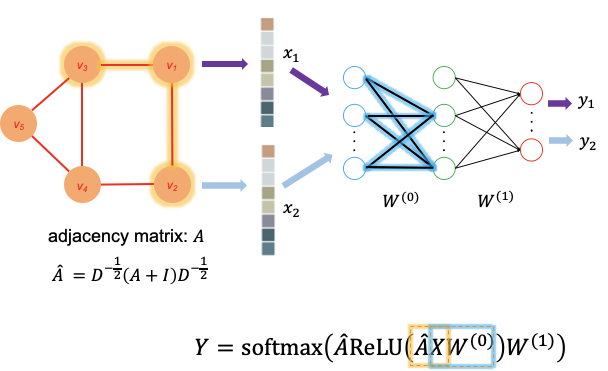
\includegraphics[scale=0.4]{pic/C3/c3_p1-3}
\caption{Illustration of  the discrete wavelet transform multi resolution analysis from 1-4 level decomposition using Haar wavelet function.}
\label{fig:c3_p1-3}
\end{figure*}

In as much as the dataset is quite small, we trained our proposed wavelet based convolution neural network (COVID-Neurowavelet) model from scratch. Several studies have reported the capability of wavelet convolution neural network for different image processing task [19], [21], and [24]. It is worth mentioning that the 4th level decomposition of our proposed model achieves quite a satisfactory result given the small amount of dataset. We believe that this work will serve as a benchmark for future works. 

\textbf{\subsection{The Proposed COVID-19 Neurowavelet}}

The proposed COVID-Neurowavelet is a wavelet convolution neural network for diagnosing COVID-19 from chest X-rays as shown in {Figure \ref{fig:c3_p1-1} }. The first three blocks have two CNN layers follow by batch normalization and ReLU activtion function whereas the fouth block has three CNN layer  follow by batch normalization and global average pool. Dropout of 0.5 is introduce in the fully connected layers for regularization. The branch  network consists of 6 convolutional layers for mapping the features of the wavelet inputs at each decomposition level into high dimensional features with samilar  filter size as the output features of each convolutional block to achieve channel-wise concatenation and dimentionality match. The proposed architecture consists of two parts.

The first part is the wavelet decomposition multi resolution analysis for image pre-processing and filtering while the second part is the convolution neural network for feature learning and classification. The first part tries to capture detailed features of the image and get rid of the noisy contents present in the image by means of a filtering technique. These high and low pass filters generate the detail and approximate components from the original image with the help of the wavelet and scaling function by down sampling with a scale factor of 2. The generated detail component is now the new input image fed to the convolution neural network for feature learning and classification. The generated approximate component is passed to the second level decomposition stage where it is further decomposed to generate a second level detail and approximate components. This process is repeated for four levels. 


The second part is subdivided into two pathways; the feature learning block and the concatenation block.  The feature learning block consists of 9 convolution layers where each convolution layer is followed by batch normalization and ReLU activation function. We did note utilize max pooling in our model rather we added global average pooling after the last convolution layers and a dropout of 50\% is added to each fully connected layer. The concatenation block consists of 3 channel-wise concatenation connected to 6 convolution layers. The first channel-wise concatenation is via a 1x1 convolution layer of 64 kernel size and second channel-wise concatenation is via two 1x1convolution layers of kernel size 64 and 128 respectively. The third channel-wise concatenation is via three  1x1  convolution layers of kernel size 64, 256 and 256 respectively. The model is trained on 20 epochs with batch of 16 and learning rate of 104 using Adam as the optimizer. The loss function adopted is the cross-entropy loss which ensures that the distance between the predicted score and the actual probability is minimized as define in {Equation \eqref{eq:1}}.

\begin{equation}
L_{CE}=-\sum_{i=1}^{N} {P_{i} log \ q_{i}}
\label{eq:1}
\end{equation}

where $P_i$ represents the actual class label and $q_i$ represents the predicted label. We adopted some evaluation metrics such as receiver operating characteristic (ROC) and precision-recall curves, area under curve (AUC), accuracy (ACC), sensitivity (SEN) and specificity (SPE). Details of the dataset utilized in the dissertation are described in subsequent headings.

\textbf{\subsection{Experiment Results}}

COVID-CXR-12 dataset is made up chest X-ray images collected from two open source dataset. We collected COVID-19 dataset from [14]. This dataset is a mixture of CT and CXR images and contains 250 CXR of COVID-19. It is important to mention that all our COVID-19 CXR is collected from this dataset. After cleaning and sorting, we arrived at a total of 162 scans of COVID-19 CXR based on the fact that only the images with observable radiographic signs are kept while every other CXR are discarded. Since the dataset repository consists of only COVID-19 and Non-COVID-19 images, we collected additional CXR of other pneumonia diseases from [15] to make up for the 12 classes. NIH dataset consists of 10,000 chest X-rays of pneumonia disease and 4,999 CXR scans of healthy patients from which we collected 162 images from each data class after thorough sorting. Table I give the number of images in COVID-CXR-12 including training, validation and test whereas Figure 2 shows the images from COVID-CXR-12.


\begin{table}[]
%\scriptsize
\centering
\caption{classification results of our proposed COVID-19 neurowavelet.}
\begin{tabular}{lllll}
\toprule
\multicolumn{1}{l}{Dataset}                     & \multicolumn{1}{l}{Accuracy (\%)} & \multicolumn{1}{l}{AUC (\%)} & \multicolumn{1}{l}{Specificity (\%)} & \multicolumn{1}{l}{Sensitivity (\%)} \\\hline
\midrule
CNN   without wavelet                             & 88                                 & 87                            & 89                                    & 90                                    \\
CNN +   1-level decomposition                     & 95                                 & 94                            & 94                                    & 95                                    \\
CNN +   2-level decomposition                     & 96                                 & 96                            & 96                                    & 97                                    \\
CNN +   3-level decomposition                     & 98                                 & 98                            & 97                                    & 99                                    \\ \hline
\multicolumn{1}{l}{CNN + 4-level decomposition} & \multicolumn{1}{l}{99}            & \multicolumn{1}{l}{99}       & \multicolumn{1}{l}{99}               & \multicolumn{1}{l}{100}  \\ \hline
\bottomrule
\end{tabular}
\label{tab2}
\end{table}

To perform a 2D discrete wavelet transform (DWT) as illustrated in Figure 3a, the images are first passed via a half-band high and low pass filters. After the filtering process, the images are sub sampled into detail and approximate coefficients using scaling and wavelet function. The images are scaled to a frequency bandwidth of π⁄2 radian using Haar wavelet function. Since the detail coefficient is characterized mainly with low frequency components, it is therefore concatenated via the channel-wise as input to the CNN block. Instead of eliminating the approximate coefficient generated in the 1-level decomposition stage simply because it consists mainly of high frequency components, it is therefore further decomposed to generate detail and approximate coefficients after undergoing the same filtering process as mentioned in the first level decomposition stage as shown in Figure 3b. The low frequency detail coefficient is concatenated via the channel-wise as input to the CNN block. 

The same process is repeated for the 3-level decomposition stage in which the approximate is further decomposed to generate a 3-level detail and approximate coefficients as seen in Figure 3c. The low frequency detail coefficient is concatenated via the channel-wise as input to the CNN block. 

Finally, as seen in Figure 3d, the further decomposition of the 3-level approximate coefficient generates a new set of detail and approximate coefficients that are aggregated as single input and concatenated via channel-wise to the CNN block. 

\textbf{\subsection{Discussion}}

This section reports the performance of COVID-Neurowavelet model on COVID-CXR-12. More importantly, we compared our proposed model in two categories: 1) we trained 4 famous pre-trained deep learning models on COVID-CXR-12 and compare their results with ours. 2) We compared our result with other image-based COVID-19 state-of-the-art models. Several studies have shown that deep learning models exhibit different converging patterns due to variations in data type and quantity. To analyze the claim, we conducted the first experiment by training our proposed CNN architecture from scratch without integrating discrete wavelet transform. From our analysis, the model achieves 88\% accuracy, 90\% sensitivity, and 89\% specificity as shown in Table II. In our second experiment, we integrated 1-level DWT decomposition into our proposed CNN architecture and the performance significantly increased at a margin of 5-6\%. The model achieves 95\% accuracy, 95\% sensitivity, and 94\% specificity as shown in Table II. From all indications, DWT has the capability to influence the convergence behavior of deep learning model during training. In our third experiment, we considered a 2-level DWT decomposition and obtained a better performance of 96\% accuracy, 97\% sensitivity, and 96\% specificity as illustrated in Table II. 

Further decomposition of the discrete wavelet transforms at the 3-level significantly increase the performance of the model by a margin of 2\% across the evaluation metrics achieving 98.5\% accuracy, 97\% specificity, and 99\% sensitivity. It is worth mentioning that our proposed model converges smoothly and fast as the decomposition level increases. The 4-level DWT decomposition shows a gentle increment in the model performance by a margin of 1\% achieving 99\% accuracy, 99\% specificity, and 100\% sensitivity as seen in Table II. Figure 4 shows the ROC curves of all the decomposition levels and their AUC values. Figure 5 presents the precision-recall curves for all decomposition levels and their average precision scores. 

\begin{table}[]
%\scriptsize
\centering
\caption{Comparison of the proposed model with state-of-the-art image based covid-19 diagnosis models.}
\begin{tabular}{lllll}
\toprule
\textbf{\multicolumn{1}{l}{Literature}}   & \textbf{\multicolumn{1}{l}{Accuracy   (\%)}} & \textbf{\multicolumn{1}{l}{Sensitivity   (\%)}} & \textbf{\multicolumn{1}{l}{Specificity   (\%)}} & \textbf{\multicolumn{1}{l}{AUC (\%)}} \\ \hline
\midrule
Wang et al {[}28{]}                    & 92.3                                 & 90.4                                    & 89.5                                    & 91.5                          \\
Shi et al {[}29{]}                     & 87.9                                 & 90.7                                    & 83.3                                    & 89.5                          \\
Jin et al {[}13{]}                     & 96.5                                 & 94.5                                    & 92.8                                    & 89.4                          \\
Xu et al {[}3{]}                       & 86.7                                 & 87.9                                    & 90.7                                    & 91.5                          \\
Wang et al {[}4{]}                     & 82.9                                 & 85.9                                    & 89.4                                    & 88.7                          \\
Barstugan et al {[}26{]}               & 90.7                                 & 91.8                                    & 92.3                                    & 95.7                          \\ \hline
\multicolumn{1}{l}{Ours   (4-level)} & \multicolumn{1}{l}{99}              & \multicolumn{1}{l}{100}                & \multicolumn{1}{l}{99}                 & \multicolumn{1}{l}{99}       \\ \hline
\bottomrule
\end{tabular}
\label{tab3}
\end{table}

The 4-level decomposition obtained the best results across all the metrics. The reason for the steady and fast convergence of our proposed model can be attributed to the fact that wavelet reduces the training load of learning the network layers that reconstruct the low frequency information. It is important to mention that the steady increase in performance of our model is as a result of the ability of wavelet to work on transform domain data in order to capture more structural details in the images to eliminate artifacts. On the bases of fair comparison, we trained 4 famous ImageNet pre-trained models on COVID-CXR-12 by fine-tuning the last layer to correspond to the number of classes in our dataset. Table IV reports the performance of these models. Figure 6 presents the ROC curves of the pre-trained models with their AUC values. 


More so, the average precision score for each pre-trained model is presented in the precision-recall curves illustrated in Figure 7. It is worth mentioning that the low performance of these pre-trained models is attributed to the size of the dataset and the complexity of the networks. At some point, these models encountered exploding and vanishing gradient problem where they could no longer learn anymore due to over saturation. This bottleneck presents our proposed model as an alternative solution to COVID-19 AI-based system in the face of data scarcity. Table III presents comparison results of previous state-of-the-art COVID-19 diagnostic models with our proposed model.

\textbf{\subsection{Comparison}}

We will present some state-of-the-art results by comparing them with our proposed model. Barstugan et al [26] proposed a technique of incorporating machine learning algorithm into deep learning network for the classification of COVID-19 from CT exams. Wang et al [27] and Xu et la [3] suggested an interesting work of detecting COVID-19 from CXR using deep learning model with few indicators. Jin et al [13] suggested a logistic regression technique to detect COVID-19. Li et al [10] proposed a dual CNN method to detect COVID-19 using CT exams. Shi et al [12] suggested a method of random forest to identify COVID-19. The findings of the aforementioned methods are presented in Table III

\begin{table}[]
%\scriptsize
\centering
\caption{Performance comparison of selected deep learning models. From all indications, the proposed wavelet integrated neural network exhibits the highest score.}
\begin{tabular}{lllll}
\toprule
\textbf{\multicolumn{1}{l}{Famous   Network}} & \textbf{\multicolumn{1}{l}{Accuracy (\%)}} & \textbf{\multicolumn{1}{l}{AUC (\%)}} & \textbf{\multicolumn{1}{l}{Specificity (\%)}} & \textbf{\multicolumn{1}{l}{Sensitivity (\%)}} \\ \hline
\midrule
VGG16                                  & 83.4                               & 89.8                          & 90.1                                  & 90.2                                  \\
Inception V3                           & 91.5                               & 84.6                          & 85.6                                  & 91.5                                  \\
ResNet50                               & 94.5                               & 87.5                          & 88.5                                  & 95.3                                  \\
VGG19                                  & 94.7                               & 86.8                          & 86.9                                  & 97.5                                  \\ \hline
\multicolumn{1}{l}{Ours   (4-level)} & \multicolumn{1}{l}{99}            & \multicolumn{1}{l}{99}       & \multicolumn{1}{l}{99}               & \multicolumn{1}{l}{100}              \\\hline 
\bottomrule
\end{tabular}
\label{tab4}
\end{table}

Reference [16] claimed that human-centered detection method of COVID-19 by radiologist using CXR could achieve high sensitivity but with very low specificity around 30\%. This low specificity usually amount to increase in false positive prediction which eventually leads to wrongly administered treatment and expense. It is obvious that our proposed model, COVID-Neurowavelet achieves a very high specificity of 99\% for the 4-level decomposition which can be considered to help expert radiologist to mitigate the reported cases of false positive. More so, the reported result in terms of Receiver Operating Characteristic (ROC) can assists expert radiologist form a balance between sensitivity and specificity.

In conclusion, it is imperative to make some commendable remarks on COVID-Neurowavelet computational cost and model complexity. By introducing wavelet transform, the use of max pool at each convolution block was eliminated thereby reducing model complexity and computational time. Another interesting advantage of our COVID-Neurowavelet is the ability to reduce noise in the input images as we concatenate the features of the generated detail coefficients and the output features of the previous convolution layer at each level of decomposition to every convolution block via 1x1convolution layer. Talking about computational cost, our model was trained for 16 minutes on NVIDIA GTX 1080. We adopted Keras framework for implementing our architecture. The model complexity of the proposed model is far reduced due to less training parameters compared to previous state-of-the-art models.

\textbf{\subsection{Conclusion}}

Our study presents the capability of multi resolution analysis for detecting COVID-19 CXR by investigating the effect of discrete wavelet transform decomposition up to 4-levels. At each decomposition level, the wavelet sub-bands are the inputs to the CNN. We put together a dataset of 1,944 CXR images of 12 classes called COVID-CXR-12 collected from two open source datasets. We trained our proposed model COVID-Neurowavelet on COVID-CXR-12 alongside other famous ImageNet pre-trained models. COVID-Neurowavelet is significantly cost-effective in terms of the number of parameters compared to the pre-trained and other state-of-the-art models and yet obtains state-of-the-art results. 


\end{document}
        % Chapter 3 inside Chapter folder
\documentclass{standalone}
% preamble: usepackage, etc.
  
\begin{document}
\chapter{Results and Discussion}
\label{Chapter4}
Image identification, classification, natural language processing, object detection, and segmentation, are the few problems that modern machine vision applications need answers to. Due to the inability of traditional machine learning to solve these complicated issue due to its strict coding constraints, deep learning approaches such as convolutional and recurrent neural networks have been introduced. It is important to mention that classical CNN models are data hungry and are unable to recognize object pose and location details, thereby prompting the development of capsule networks. 

The expectation of capsule networks in connection with all of the aforementioned problems, outperforms CNN models. Despite this promising performance, researchers are yet to fully exploit its advantages due to the lack of architectural information and understanding of the working principles of capsule network. Recently, some deep learning models are utilizing capsule networks as its primary back bone framework ever since it was introduced. The most widely used form of capsule network employs a layer-to-layer routing method known as "routing by agreement." In CNNs, this approach substitutes pooling and scalar outputs with a vector output. The size of the output denotes the probability that an attribute depicted by the capsule is present in the input, while the object's position denotes the instantiation variable.


%%%%%%%%%%%%%%%%%%%%%%%%%%%%%%%%%%%%%%%%%%%%%%%%%%%%%%%%%%%%%%%%%%%%%%%%%%%%%%%% Paper 2 %%%%%%%%%%%%%%%%%%%%%%%%%%%%%%%%%%%%%%%%%%%%%%%%%%%%%%%%%%%%%%%%%%%%%%%%%%%%%%%%%%%%%%%%%%%%%%%%

\textbf{\section{Shared Weighted Continuous Wavelet Capsule Network for Electrocardiogram Biometric Identification}} 

Despite various usability and security issues, conventional passwords remain the most used method of internet authentication [1]-[3]. Passwords are inconvenient for users since they must be remembered and preferably, be lengthy and distinct. As a result, it should come as no surprise that many users choose weak passwords that they reuse across several platforms [4], [5], resulting in account hack and personal data breaches. According to studies, over 50\% of users use the same authentication credentials for several platforms [4] and over 80\% of privacy breaches are caused by poor authentication credential behavior [6]. 

Alternative authentication techniques, such as push notifications [7], graphical passcodes [8], and trust scores [9], and gestures [10], have been investigated in attempt to replace or supplement standard passwords. Biometric authentication is of particular importance due to its unique characteristics of user identity. Biometrics enhances usability of the system by eliminating the need for users to remember passwords or move about with a token at all times. The simplicity with which biometrics can be used for authentication has sped up their adoption in both the private and public sectors, with the global market for biometric technology anticipated to hit \$59.31 billion by 2025 [11].

While much of the previous research has focused on standard biometrics like fingerprints, facial recognition, and iris scans, there has been little work done to investigate new biometrics. In this paper, we look at a biometric based on electrocardiogram (ECG) signals, which represent the electrical activity of the human heart. ECG has been shown to be adequately unique to every person in previous studies [12] and could be utilized for identity verification. In this paper, we proposed a hybrid scheme of continuous wavelet transform (CWT) and capsule network for biometric authentication based on ECG.CNN has made significant progress in a variety of applications, particularly in detecting anomalies in radiographs [13] – [16]. 

%\begin{figure*}[t!]
%\centering
%\includegraphics[scale=0.1]{C4/c4_p2-1}
%\caption{Proposed scheme for detecting DDoS attack on smart grid.}
%\label{fig:c4_p2-1}
%\end{figure*}

While biometrics are more usable than standard passwords, there are still issues about biometric data security and privacy [17]. Biometrics cannot be readily reversed once they have been infiltrated, as they are based on an individual's lasting physiological or behavioral features. Additionally, biometric recognition system operators may gain undesired information from a user's biometric data. Fingerprint patterns, for example, may be linked to certain disorders [18]. In conclusion, some biometric traits, such as a person's face, are difficult to conceal. As a result, even if a person wants to remain unknown, they may be recognized without their consent or knowledge [18].

The heart is a muscular organ that supplies blood to the body's tissues via blood vessels [19]. The heart muscle must contract in order to supply blood, resulting in an electrical impulse. During an electrocardiogram (ECG) examination, this impulse can be measured on the surface of the body using electrodes put on the skin. The process of depolarization and repolarization of the heart chambers, which causes them to contract and rest, is captured by an ECG tracing.

%\begin{figure*}[t!]
%\centering
%\includegraphics[scale=0.1]{C4/c4_p2-2}
%\caption{Conversion of one-dimensional traffic data to two-dimensional images using CWT.}
%\label{fig:c4_p2-2}
%\end{figure*}

Various researchers have looked into the ECG's peculiarity and stability. The majority of these are based on a "on-the-person" approach "a method for signal acquisition in which electrodes are placed directly on the person [20]. There are limited researches that use "off-the-person" methodology "They use a different approach, but they show a real-life application scenario for ECG identification systems. Placing ECG sensors into a smartphone cover, wristbands, and car steering wheel are just a few instances. Additionally, as shown in [20], previous researches frequently employ data acquired from a single data acquisition session which are easy to develop. 

In this work, CWT is utilized to convert the 1-dimensional time-series signal of ECG to 2-dimensional time-frequency scalogram as input image of distinct features with growing sensitivity which makes it suitable for CNN model to extract feature for training. The image features obtained from CWT are utilized to train the proposed capsule network for biometric authentication. We adopted some well-known evaluation metrics to validate the performance of the proposed scheme. 
Conclusively, we assess the effectiveness of the proposed scheme using public dataset and also presented some comparison with other methods of biometric authentication.

\textbf{\subsection{Methodology}} 
The proposed method for biometric identification using ECG is described in this section. Figure 1 depicts the general framework of the proposed scheme for user identification. First, the dataset utilized in this study for ECG biometric identification is properly described. 

\textbf{\subsubsection{Dataset}} 

Instead of creating a new dataset, we used an already existed dataset. For this study, we used the MIT-BIH Normal Sinus Rhythm available on Physionet database. The Physionet MIT-BIH Normal Sinus Rhythm database consists of healthy ECG records of persons between the ages of 20 and 50 with no major arrhythmias collected at the Arrhythmia laboratory of Boston’s Beth Israel Hospital[21]. Compared to other ECG dataset, Physionet MIT-BIH dataset has been utilized by most studies. Physionet MIT-BIH dataset consists of 30 recordings of normal sinus rhythm signals.

\begin{figure*}[t!]
\centering
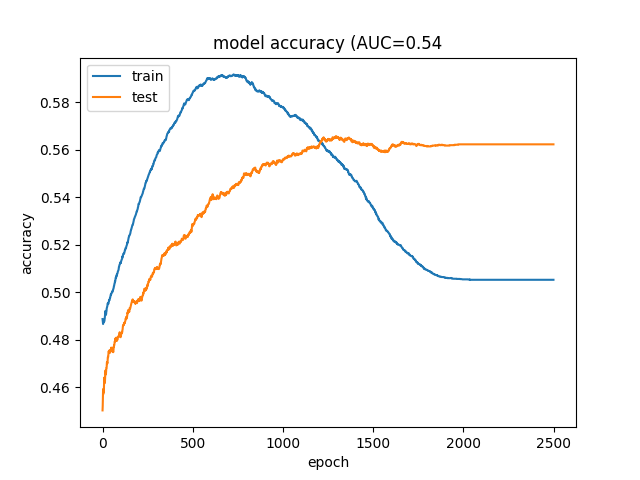
\includegraphics[scale=0.4]{C4/c4_p2-3}
\caption{Proposed wavelet convolutional neural network for detecting DDoS attack on smart grid infrastructure.}
\label{fig:c4_p2-3}
\end{figure*}

\textbf{\subsubsection{Proposed siamese capsule network (WavCapNet)}} 

This research proposes a siamese capsule network, as shown in Figure 3. The model accepts two scalogram images as inputs, and then transmits them into a shared weighted framework. The obtained data is forwarded into the fully-connected layer, and the model then determines if the outcome is valid or invalid. Our proposed model's method is based on a real-world security assessment of person identity.

In a real-world scenario, tenants of a specific building or employees of a company with access control security equipment are normally asked to go through a security check. These persons' biometric templates must have been stored in the system. When a person attempts to enter an authorized building or organization, a comparison of both the template and the query input is performed to determine whether the request is valid or invalid. As a result, the idea of employing a siamese capsule network to receive both ECG trait images, access their attributes, and determine whether they are similar or not is proposed. In general, a siamese network is used to compare two input images with similar weights and parameters. The extracted feature vectors of the two inputs are then obtained from the last layer, and the Euclidean distance is computed. If the distance between the two images is large, they are different, otherwise, they are similar.


Computing the similarity of the ECG images will be omitted in our investigation, and instead the relationship between the two images will be utilized to predict the outcome. As a result, the distance calculating aspect of our work is eliminated, as shown in Figure 3. For feature extraction, a shared weighted capsule network with modified AlexNet as the base neural network is used, then the retrieved features are fused and passed into the fully-connected layer, and ultimately, the ECG images are predicted using a sigmoid classifier. Instead of the usual max-pooling layer, we introduced discrete wavelet pooling to replace the first and second max-pooling layers for down-sampling operation whereas the third max-pooling layer is eliminated to arrive at a feature vector of $256 \times 14 \times 14 $. The likelihood of which ECG trait matches the query or not is represented by the prediction result which is either 0 or 1.

\textbf{\subsubsection{Experimental detail and setup}} 

The basic technique of the proposed scheme is split into two phases: data pre-processing and feature extraction. The pre-processing step begins with the collection of raw ECG signals from the Physionet database. The most essential and consistent fundamental characteristics are obtained in the pre-processing step by converting one-dimensional time domain ECG signal to time-frequency domain image of two-dimension using CWT. This work employed continuous wavelet transform and siamese wavelet capsule networks trained on Physionet MIT-BIH ECG dataset for biometric identification using Adam optimizer and dropout to prevent over-fitting, early stop strategies, and a learning rate of $10^{4}$ to improve performance. Keras library with Tensorflow as the backend on a GeForce GTX 1080 GPU is used for the implementation of this work. Accuracy, sensitivity, specificity and AUC are some of the evaluation metrics applied on our proposed model. 

\begin{table}[]
\caption{Performance comparison of our proposed model with selected pre-trained models.
WavCovNet model.}
\begin{tabular}{lllll}
\toprule
\multicolumn{1}{l}{Model} & \multicolumn{1}{l}{ACC (\%)} & \multicolumn{1}{l}{SEN (\%)} & \multicolumn{1}{l}{SPE (\%)} & \multicolumn{1}{l}{Time (Min)} \\ \hline
\midrule
ResNet-101                  & 95.7                         & 95.8                         & 94.6                         & 47                              \\
EfficientNet                & 94.7                         & 94.3                         & 95.8                         & 40                              \\
MobileNet-V3                & 95.2                         & 94.5                         & 95.9                         & 39                              \\
DenseNet                    & 96.6                         & 95.4                         & 96.3                         & 46                              \\ 
\multicolumn{1}{l}{Ours}  & \multicolumn{1}{l}{99.2}    & \multicolumn{1}{l}{98.6}    & \multicolumn{1}{l}{99.5}    & \multicolumn{1}{l}{48}         \\ \hline
\bottomrule
\end{tabular}
\label{tab6}
\end{table}


\textbf{\subsubsection{Results and discussion}} 
The proposed ECG biometric identification scheme is built using the Keras framework and Tensorflow as the backend. We examined the proposed strategy for ECG biometric identification based on binary classification for both query match and mismatch in security access control systems during training and validation. The proposed approach obtains 99.2\% accuracy rate for identifying query match and mismatch. The proposed model's training and validation accuracy curves are depicted in Figure 4, which show that the model converges smoothly without over-fitting. The proposed scheme's training and validation loss curves are gradually and steadily reduced as shown in Figure 5. In general, the proposed siamese wavelet capsule network's performance is reasonable. It's crucial to evaluate the proposed model's validity using the receiver operating characteristic curve (ROC), which depicts the proposed scheme's overall accuracy in terms of area under the curve (AUC). Figure 6 illustrates that the proposed scheme has a high sensitivity combined with a high specificity, resulting in a low false positive rate and a high true positive rate.



As shown in Table 1, our proposed approach obtains 98.6\% sensitivity and 99.5\% specificity. The results of our proposed scheme versus certain pre-trained models are shown in Table 1. When it comes to correctly determining query match and mismatch of ECG characteristics, the proposed strategy clearly outweighed the selected pre-trained techniques by 2.6\% in terms of accuracy. In addition, the proposed method achieved 2.6\% increase in sensitivity and 3.2\% increase in specificity when compared to pre-trained procedures. EfficientNet had the lowest accuracy (94.7\%) and sensitivity (94.3\%) scores, whereas ResNet-101 had the lowest specificity score (94.6\%). It is worth noting that the proposed scheme has a slightly higher computational time of about 48 minutes in training but achieves the best result, as shown in Table 1. Though MobileNet-V3 had the shortest training time of 39 minutes, our proposed model still achieves satisfactory performance. 

\textbf{\subsubsection{Conclusions}} 

Biometric identification systems provide several benefits that traditional techniques do not. We proposed an ECG-based biometric identification system for security access control in this research, in which a continuous wavelet transform (CWT) was utilized to convert one-dimensional time-domain signals into scalograms of two-dimensional images to obtain good quality training data. A siamese capsule network framework was utilized to predict the right match or mismatch of ECG query samples using the extracted specific attributes from the scalograms. The findings show that the ECG signal is a reliable biometric measure that is resistant to noise and artifacts. Furthermore, the proposed security system's efficiency was assessed using both classification metrics and the ROC-AUC measure. The proposed scheme properly predicted ECG query samples with 99.2\% accuracy, which is 2.6\% higher than the other models.





%%%%%%%%%%%%%%%%%%%%%%%%%%%%%%%%%%%%%%%%%%%%%%%%%%%%%%%%%%%%%%%%%%%%%%%%%%%%%%%%%%%%%%%%%%%%%%%%%%%%%%
\end{document}        % Chapter 4 inside Chapter folder
\documentclass{standalone}
% preamble: usepackage, etc.
\begin{document}
\chapter{Conclusion}
\label{Chapter5}
Due to the obvious increased output of large amounts of information in recent times, particularly images, it is becoming necessary to build techniques and software for the automatic collection, processing, and analysis of such information in order to extract trends and patterns. This guarantees that images and its characteristics are converted by algorithm into representations that reflect their context and interpretation. Currently, innovations in artificial intelligence are being applied to system algorithms for image analysis and complicated analysis in the field of machine vision. Image classification and recognition are essential components of machine vision. These activities are simple for humans, but they require complicated numerical concepts and advanced computational procedures for machines to execute. This dissertation presents wavelet multi-resolution analysis and deep learning model combined into a single framework for image recognition and classification, with up-to-date results on the MIT-BIH normal sinus rhythm, case western reserve university, COVID-19 radiograph database, CICDDos2019, NIH pneumonia, RSNA pneumonia and CT-datasets, respectively.


\textbf{\section{Research Findings}}
In this dissertation, we examined the application of wavelet multi-resolution analysis and deep learning models as a single framework for the task of machine fault diagnosis, biometric identification and disease classification. We recognize the importance of decreasing the discrepancy between computer and human judgment, therefore we have designed models that contributes to the advancement of artificial intelligence, particularly in machine vision.

\textbf{\section{Contributions}}
In this dissertation, we presented wavelet multi-resolution analysis algorithm and deep learning model as a single framework capable of attaining and advancing the horizon of research in medical imaging, machine fault diagnosis and biometric identification. We believe that this advances the requirement for intelligent data analysis, interpretation, and augmenting a limited human reliance on image interaction and understanding.


\textbf{\section{Future Works}}
Given the vast amount of research in vision recognition and image classification, there are still a number of obstacles to overcome before reaching same accuracy of that of human. To begin, our models are supervised framework, which necessitates a large quantity of data to learn the mapping from an input $X$ to a label $Y$. This type of learning domain necessitates a lot of human tagging and labeling, which makes the process difficult and resource-intensive from a computational and hardware standpoint. Designing models that acquire intuitive representation without the need for limitless training sets is a viable solution.


\end{document}        % Chapter 5 inside Chapter folder

% The diagrams/images that corresponds to each chapter are arranged 
% in a separate folder inside the Pic folder. 


%\documentclass{standalone}
% preamble: usepackage, etc.
\begin{document}
	
前方高能,非战斗人员请撤离
弹幕  护体
弹幕  护体
弹幕  护体
弹幕  护体


\begin{landscape}
\begin{table}[t]
\caption{System corrections of the learning strategies for a relatively longer test sentence}
\label{table4}       % Give a unique label

\begin{tabular}{p{6cm} p{13cm}  } %{ll|l|l|l|l}

\hline
\hline
\textbf{System} & \textbf{Sentence}  \\
\noalign\hline
Source    
&But I disegree this opinion because often the advertisement do n't speak about the only functionals of the product but it promises other characteristics that do n't depend by it .   \\

\hline\hline
Two-tier seq2seq \(\Theta_{B_0}\leftarrow\Theta_{B_1}\), \(S^*\)                     
&But I \textcolor{red}{agree} this opinion because often the advertisement do n't speak about the only functionals of the product but it promises other characteristics that do n't depend by it .   \\

\hline
Three-tier seq2seq  \(\Theta_{B_0}\leftarrow\Theta_{B_1}\leftarrow \Theta_{B_2}\), \(S^*\)    
&But I \textcolor{blue}{disagree with} this opinion because often the advertisement do n't speak about the only functionals of the product but it promises other characteristics that do n't depend by it . \\

\hline
Two-tier seq2seq \(\Theta_{B_0}\leftarrow\Theta_{X}\), \(S^*\)      
&But I \textcolor{red}{agree} \textcolor{blue}{with} this opinion because often the advertisement do n't speak about the only functionals of the product but it promises other characteristics that do n't depend by it .\\

\hline
Three-tier seq2seq \(\Theta_{B_0}\leftarrow\Theta_{X}\leftarrow \Theta_{Y}\), \(S^*\)	     
&But I \textcolor{blue}{disagree with} this opinion because often the advertisement do n't speak about the only functionals of the product but it promises other characteristics that do n't depend by it .  \\

\hline\hline

Two-tier seq2seq \(\Theta_{B_0}\leftarrow\Theta_{B_1}\), \(S^{**}\)		               	        
&But I \textcolor{blue}{disagree with} this opinion because often the \textcolor{blue}{advertisements} do n't speak about the only \textcolor{blue}{functions} of the product but it promises other characteristics that do n't depend by it . \\

\hline
Three-tier seq2seq \(\Theta_{B_0}\leftarrow\Theta_{B_1}\leftarrow \Theta_{B_2}\), \(S^{***}\)		    
&But I \textcolor{blue}{disagree with} this opinion because often the \textcolor{blue}{advertisements} do n't speak about the only \textcolor{blue}{functions} of the product but it promises other characteristics that do n't depend \textcolor{blue}{on} it .   \\

\hline
Two-tier seq2seq  \(\Theta_{B_0}\leftarrow\Theta_{X}\), \(S^{**}\)			                     
&But I \textcolor{blue}{disagree with} this opinion because often the \textcolor{blue}{advertisements} do n't speak about the only \textcolor{blue}{functions} of the product but \textcolor{red}{it fails to express others .} \\

\hline
Three-tier seq2seq \(\Theta_{B_0}\leftarrow\Theta_{X}\leftarrow \Theta_{Y}\), 
\(S^{***}\)			
&But I \textcolor{blue}{disagree with} this opinion because often the \textcolor{blue}{advertisements} do n't speak about the only \textcolor{blue}{functions} of the product but \textcolor{red}{it fails to express others .} \\

\hline\hline
Reference 0	   &But I \textcolor{blue}{disagree with} this opinion because often the advertisement \textcolor{blue}{does n't} speak about only the \textcolor{blue}{functionality} of the product , but it promises other characteristics that do n't depend \textcolor{blue}{on} it .  \\

\hline
Reference 1	  &But I \textcolor{blue}{disagree with} this opinion because often the \textcolor{blue}{advertisements} do n't speak about the only \textcolor{blue}{functions} of the product , but it promises other characteristics that they do n't deliver \textcolor{blue}{on} .  \\

\hline
Reference 2	  &But I \textcolor{blue}{disagree with} this opinion because often the advertisement \textcolor{blue}{does n't} speak about the \textcolor{blue}{function} of the product but it promises other characteristics that do n't depend \textcolor{blue}{on} it .  \\

\hline
Reference 3	  &But I \textcolor{blue}{disagree with} this opinion because often the advertisement \textcolor{blue}{does n't} just speak about the \textcolor{blue}{functionality} of the product but it promises other characteristics that do n't depend on it .  \\
\noalign{\smallskip}\hline\hline\noalign{\smallskip}

\multicolumn{2}{l}{Note: }\\
\multicolumn{2}{l}{{\(S^*\) - The model was trained with the NUCLE dataset.}}\\
\multicolumn{2}{l}{{\(S^{**}\) - The model was trained with the NUCLE and FCE datasets }}\\
\multicolumn{2}{l}{{\(S^{***}\) - The model was trained with NUCLE, FCE
and Lang-8 datasets.}}
\end{tabular}
\end{table}
\end{landscape}

\end{document} %若需添加第六章请用这个模板修改

% misc
\documentclass{standalone}
% preamble: usepackage, etc.
\begin{document}

\thesisacknowledgement
First and foremost, I want to express my gratitude to my supervisor, Professor Jian Ping Li, who transformed me into a successful researcher through his patience, advice, and rigorous tutoring. Your prompt suggestions and counsel guided me in the right route, allowing me to achieve my PhD ambitions. I appreciate your confidence in me and the pleasant relationship you established with me during my academic years. I have learned a great deal from you, not only in terms of academics, but also in terms of overall development.

My research partner, Grace Ugochi Nneji, has been a huge source of inspiration for me over the last few years. Your regular motivation, interactions, and remarks influenced the direction of my studies and pushed me to achieve more. Your contributions were important elements of my foundation. It has also been a great pleasure to work with my Wavelet Analysis and Active Media Technology and Big Data Research Lab colleagues. Your suggestions and participation have helped to make my journey memorable and productive.

In addition, I owe a debt of appreciation to certain friends who have had a significant impact on my life. This includes Ariyo Oluwasanmi, Folarin Mordecai Raji, and Akeem Shokanbi. Your wishes, support, and care created an environment that was positive and conducive to my mental and physical health. Thank you for being such a wonderful people.

Thank you to UESTC's International Student Education Office and the entire School of Computer Science and Engineering. Finally, I would like to offer my heartfelt appreciation to my family for their unwavering support. During the difficult moments, I find consolation in your love and wishes. I owe everything I am to my late mother who was always willing to help me become the man of my dream.


\end{document}  %致谢
\thesisloadbibliography[nocite]{reference}  %参考文献


% comment while no need
%\documentclass{standalone}
% preamble: usepackage, etc.
\begin{document}

\thesisappendix

\end{document}   %附录,论文若无附录则用%将该命令取消
\thesisloadachievement{publications}  %攻读学位期间取得的成果,若无成果则用%将该命令取消
%\documentclass{standalone}
% preamble: usepackage, etc.
\begin{document}

\thesistranslationoriginal
\section{A Tight Upper Bound on Bit Error Rate}

\end{document}  %外文资料原文,论文若未引用外文资料则用%将该命令取消
%\documentclass{standalone}
% preamble: usepackage, etc.
\begin{document}

\thesistranslationchinese
\section{基于多载波索引键控的正交频分多路复用系统模型}

\end{document}   %外文资料译文,论文若未引用外文资料则用%将该命令取消

\end{document}
